\section{Enclave Operation}

SGX provides trustring computing by protecting the privacy and integrity of the
computation that is performed inside an enclave, and by providing remote
attestation identifying the software running inside an enclavee. This section
describes the processes used to set up an enclave and perform computation
inside it.

\subsection{Enclave Setup}



\subsection{Evicting EPC Pages}
\label{sec:sgx_ewb}

% Eviction of Enclave Pages: SGX S 3.5.3

% EPA: SGX S 5.3 EPA

\begin{figure}[hbt!]
  \center{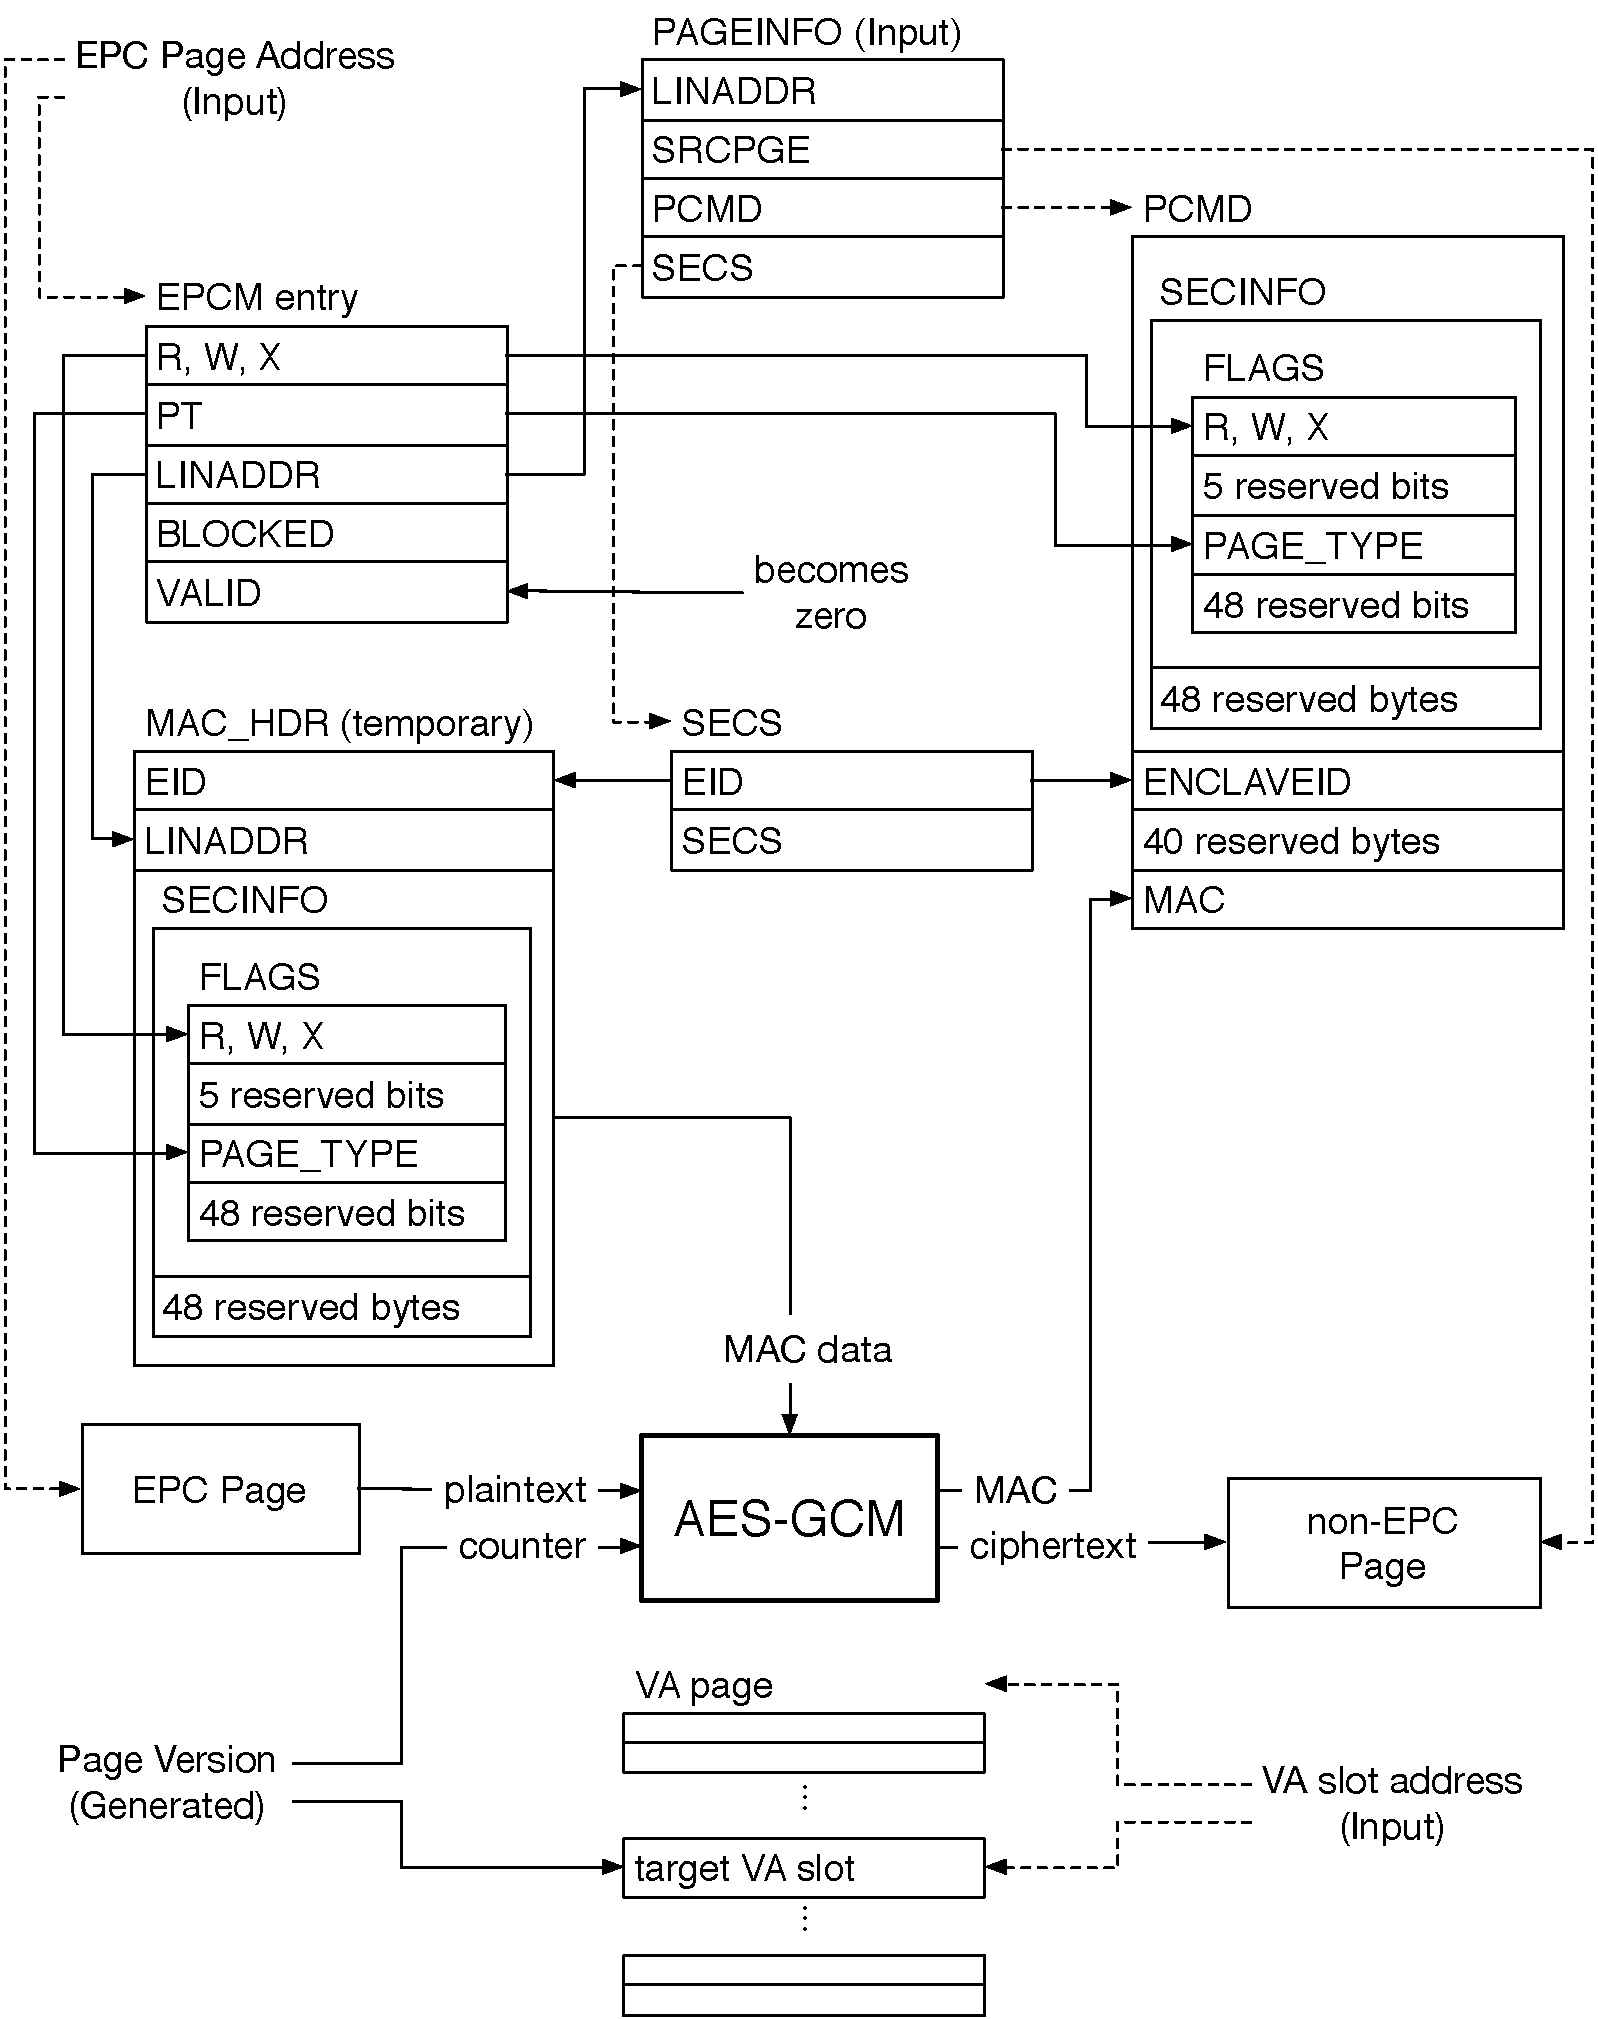
\includegraphics[width=85mm]{figures/sgx_ewb.pdf}}
  \caption{
    The data flow of the EWB instruction that evicts an EPC page. The page's
    content is encrypted in a non-EPC RAM page. A nonce is created and saved
    in an empty slot inside a VA page. The page's EPCM metadata and a MAC
    are saved in a separate area in non-EPC memory.
  }
  \label{fig:sgx_ewb}
\end{figure}

% Loading an Enclave Page: SGX S 3.5.4

